% =====================================================================
% Conference paper in ieeeconf format, targeting ECC. 6-page limit.
%
% FRAMING (settled): the paper's object is the LIMIT CYCLE of fixed-step
% and accelerated SPIN tuning. The triple point is the tool that locates
% the cycle's center; the regularized index is the tool that makes the
% analysis well posed. Neither appears in the title.
%
% Numbers policy: all from verified follow-up runs. TODO-REGEN entries
% need regeneration before submission; TODO marks editorial placeholders.
% =====================================================================
\documentclass[letterpaper, 10pt, conference, twocolumn]{ieeeconf}

\usepackage{amsmath,amssymb,amsthm}
\usepackage{graphicx}
\usepackage{booktabs}

\newtheorem{proposition}{Proposition}
\newtheorem{corollary}{Corollary}
\newtheorem{lemma}{Lemma}
\newtheorem{observation}{Observation}
\newtheorem{remark}{Remark}

\newcommand{\Nbar}{\bar{N}}
\newcommand{\Neps}{N_{\varepsilon}}

% Paper title
\title{Limit Cycles of Model-Free PID Tuning by Step-Response Inspection}

% Author names and affiliations
\author{Pavel Otta$^{1}$, Daniel Pachner$^{1}$, Ji\v{r}\'{\i} Dost\'al$^{1}$
and Vladim\'{\i}r Havlena$^{2}$%
\thanks{$^{1}$University Centre for Energy Efficient Buildings (UCEEB),
Czech Technical University in Prague, Bu\v{s}t\v{e}hrad, Czech Republic.
Corresponding author: \texttt{pavel.otta@cvut.cz}}%
\thanks{$^{2}$Department of Control Engineering, Faculty of Electrical
Engineering, Czech Technical University in Prague, Prague, Czech Republic.}%
}

\begin{document}

\maketitle

\begin{abstract}
In a companion paper we introduced SPIN, a model-free method for tuning
PID controllers. It draws three phase portraits from one closed-loop
step response, counts a turn index in each, and then changes the gains
using a fixed table of four moves and a constant step size. The
iteration does not stop at a point. It ends in a small periodic orbit.
This paper explains that orbit. We show that it is not an accident but a
property of the rule. In log-gain coordinates the four moves have
exactly one convex combination that sums to zero. This forces the orbit
to circle the \emph{triple point}, the gain vector at which all three
turn indices sit exactly on their thresholds, and it fixes the move
frequencies at $(\tfrac18, \tfrac12, \tfrac14, \tfrac18)$. Measured
frequencies agree to three decimal places. The same computation over the
integers shows that the shortest possible orbit has length eight, and
the observed orbit is a binary counter on the corners of a cube of side
$\log\gamma$ centered on the triple point. To state all this properly we
replace the published integer count by an $\varepsilon$-regularized
winding integral, used here only as a tool for the analysis. The theory
gives a direct practical result. Since the cube is aligned with the gain
axes, a fixed step $\beta$ keeps every gain within the factor
$(1-\beta)^{-1/2}$ of the target set by the plant. A tolerance $\rho$ per
gain is therefore met by choosing $\beta \le 1-\rho^{-2}$, and the
companion paper's default $\beta = 0.1$ guarantees $5.4\,\%$ per gain.
Finally, a schedule that halves the step once every band has reversed
shrinks the cube geometrically and reaches $10^{-4}$ accuracy in fewer
than a hundred iterations.
\end{abstract}

\begin{IEEEkeywords}
PID control, model-free tuning, limit cycles, switched systems,
winding number
\end{IEEEkeywords}

% =====================================================================
\section{Introduction}
\label{sec:intro}

Most PID tuning methods first fit a model and then compute the gains
\cite{ZN1942,AstromHagglund2004}. In a companion paper \cite{Paper1} we took a
different route and tuned directly from what the step response \emph{looks
like}. The method is called SPIN (Step-response Phase-portrait INspection). It
draws three phase portraits from one closed-loop step response and counts how
many times each curve turns around the origin. This count is the \emph{turn
index} $N_k$ of band $k$, and it is compared with a fixed threshold. A table of
four moves, the \emph{triangular rule}, then scales the gains up or down by a
constant factor. No plant model is identified at any point.

The companion paper shows that the rule detunes aggressive gains, recovers
from failed loops, and reaches a feasible region on a battery of standard
plants. It also reports one behavior that it does not explain. No run stops at
a point. Every successful run ends in a small periodic orbit in gain space.
That orbit is the subject of this paper, and we ask four questions about it.

\emph{Where is it?} Which point does the orbit circle, and is that point
fixed by the plant or by the history of the run? \emph{What is its shape and
size?} Which moves occur, in what proportion, how short can an orbit be, and
can the step size be chosen to meet a required accuracy on the gains?
\emph{Why this rule?} The moves are a design choice in the companion paper;
is another choice possible? \emph{Can the orbit be made smaller?} Is there a
faster schedule whose accuracy the theory can guarantee rather than only
observe?

One technical step comes first. The published turn index is an integer count,
so it is discontinuous in the gains, and the boundaries between the regions of
the rule are then not well defined. Section~\ref{sec:index} replaces it by an
$\varepsilon$-regularized winding integral. This is a tool for the analysis and
not a change to the method: every sign comparison made by the published rule
stays the same.

Our answers are then as follows. The orbit circles one point that depends only
on the plant. We call it the \emph{triple point}, because all three turn
indices sit exactly on their thresholds there (Section~\ref{sec:cycle}). The
move frequencies and the shortest possible length of eight both follow from a
single balance condition on the four moves, and the orbit is a binary counter
on the corners of a cube of side $\log\gamma$. The move table itself is forced:
it is the only one compatible with the priority logic
(Section~\ref{sec:why}). The shape of the cube gives a simple formula for
choosing the step size from a required gain accuracy (Section~\ref{sec:size}).
Finally, a schedule that halves the step after every band has reversed shrinks
the orbit geometrically and reaches $10^{-4}$ accuracy in fewer than a hundred
iterations (Section~\ref{sec:accel}).

Iterative model-free tuning is not new. Iterative feedback tuning
\cite{Hjalmarsson1998} and extremum seeking \cite{Killingsworth2006} both
estimate the gradient of a cost from closed-loop experiments and converge to a
local minimum of it. The triangular rule is different: it uses only
\emph{signs}, with no cost function and no gradient. Its natural end state is
therefore not a stationary point but a limit cycle of a switched system, which
is exactly what averaged (Filippov) dynamics were developed for
\cite{Filippov1988}.

% =====================================================================
\section{The Rule as a Switched System}
\label{sec:rule}

We recall only what is needed; the companion paper \cite{Paper1} defines the
portraits, the index, and the rule in full. One closed-loop step experiment
yields three curves (band $0$, $1$, $2$), and for each curve a turn index
$N_k \ge 0$ measuring how far the curve winds around the origin of its
portrait. Each band has a fixed threshold:
\begin{equation}
\Nbar = (\Nbar_0, \Nbar_1, \Nbar_2) = (0.5,\; 0.75,\; 1.0).
\label{eq:thresholds}
\end{equation}

The triangular rule reads the three comparisons $N_k \gtrless \Nbar_k$ and
applies one of four moves to the gain vector. Following \cite{Paper1} we
order the gains by the band each channel dominates,
$K^{(0)} = K_i$, $K^{(1)} = K_p$, $K^{(2)} = K_d$, so that $N_k$ is the index
pointing at $K^{(k)}$. If all
three bands are below threshold, all gains are scaled up; otherwise the lowest
offending band is cut by scaling gains down in a band-specific pattern. Every
move multiplies each gain by $\gamma^{\pm 1}$ or leaves it alone, where
$\gamma = 1/(1-\beta)$ and $\beta$ is the step size (default $\beta = 0.1$,
so $\gamma \approx 1.111$). Multipliers are clipped to a box, here
$[0.01, 10]$.

Throughout we assume the step response is measured without output noise, so
that each turn index is a deterministic function of the gains. The stochastic
case, in which the three comparisons become random near the target, is treated
in follow-up work; the deterministic characterization below is its zero-noise
limit, and Proposition~\ref{prop:unique} records a combinatorial property of
the move table that bears on it.

We use log coordinates $\theta = (\log K_i, \log K_p, \log K_d)$. Note that
these are in band order and not in the usual PID order. The four moves are then
translations by $h = \log\gamma$:
\begin{equation}
\begin{aligned}
e   &= (+1, +1, +1) &\text{(expand),}\\
d_0 &= (-1, \phantom{+}0, \phantom{+}0) &\text{(cut band 0),}\\
d_1 &= (+1, -1, \phantom{+}0) &\text{(cut band 1),}\\
d_2 &= (+1, +1, -1) &\text{(cut band 2),}
\end{aligned}
\label{eq:moves}
\end{equation}
each scaled by $h$. The iteration is therefore a switched dynamical system.
The signs of $N_k(\theta) - \Nbar_k$ divide gain space into four regions, and
each region is given one constant velocity. Since the velocity never vanishes
inside a region, the state can never come to rest. A bounded trajectory must
keep crossing from one region to another, so the rule must end in a cycle. Two
questions remain: where the regions meet, and how the crossing pattern arranges
itself there. Section~\ref{sec:index} makes the first question well posed, and
Section~\ref{sec:cycle} answers both.

% =====================================================================
\section{A Continuous Index for the Analysis}
\label{sec:index}

Both questions concern the boundaries between regions, so before either can be
answered we must check that those boundaries exist. With the turn index as
published they do not. That index is a hard count: the
winding is accumulated along the portrait curve and then cut off when the curve
enters a small disc of radius $\varepsilon$ around the origin for the last
time. The time of this \emph{last entry} does not depend continuously on the
curve. A very small change can make the curve just touch the edge of the disc,
and one whole turn is then gained or lost. On the battery plants a gain change
of $0.05\,\%$, far smaller than any step the rule takes, moves one index by
exactly $1.000$, and a longer simulation window does not help. The switching
surfaces $N_k(\theta) = \Nbar_k$ are then not surfaces at all, the four regions
of Section~\ref{sec:rule} have no well-defined boundaries, and no statement
about where they meet can even be formulated.

For running the rule this jump does no harm. The rule reads only the
\emph{sign} of $N_k - \Nbar_k$, and a jump of one simply moves a switching
surface a little. This is why all results of the companion paper remain valid.
The analysis, however, needs a continuous index, and there is a natural one.
For a curve $(x(t), y(t))$ we replace the hard cut-off by a smooth weight:
\begin{equation}
\Neps \;=\; \frac{1}{2\pi} \oint
\frac{x\,dy - y\,dx}{\,x^2 + y^2 + \varepsilon^2\,}.
\label{eq:neps}
\end{equation}
Write $\rho^2 = x^2 + y^2$. The integrand is then the usual winding integrand
multiplied by the weight $\rho^2 / (\rho^2 + \varepsilon^2)$. Turning far from
the origin counts fully, turning at radius $\varepsilon$ counts half, and
turning deep inside the disc counts almost nothing. Three properties make
$\Neps$ the right tool.

\emph{It is continuous.} The integrand is smooth everywhere, so $\Neps$ is a
continuous function of the gains. For the $0.05\,\%$ change above it moves by
$7 \times 10^{-4}$, where the hard count jumps by $1.000$.

\emph{It does not depend on the window.} After the response has settled the
radius tends to zero, and there the weight tends to zero as $\rho^2$. The value
of $\Neps$ is therefore exactly independent of the window length, and the
$\delta$-guard of the hard count is no longer needed.

\emph{It can replace the count.} Away from the switching surfaces $\Neps$ and
the hard count agree up to an error that tends to zero with $\varepsilon$.
Every sign comparison of the published rule is therefore unchanged, and so is
every published result.

With $\Neps$ the sets $N_k(\theta) = \Nbar_k$ are true level surfaces, and the
analysis of the next section is well posed. We also check directly that these
surfaces meet in a single point. Runs in which the step size is driven to zero,
which is a device for the analysis and not a tuning recommendation, converge to
that point, which Section~\ref{sec:cycle} calls $\theta^*$, with final log-gain
errors
\begin{equation*}
\text{P1: } 0.010, \quad \text{P3: } 0.017, \quad \text{P4: } 0.041,
\end{equation*}
where $\theta^*$ is located independently by direct search on
\eqref{eq:triplepoint}. With the hard count the same runs stop at points that
depend on the schedule. This is further evidence that only the regularized
index reveals the true center of the cycle.

% =====================================================================
\section{The Limit Cycle and Its Center}
\label{sec:cycle}

We now use the regularized index of Section~\ref{sec:index} throughout, so
that the four regions have genuine boundaries. Suppose a trajectory stays
bounded and does not drift. Over a long window,
each move $v \in \{e, d_0, d_1, d_2\}$ is applied some fraction $w_v \ge 0$ of
the time, with $\sum_v w_v = 1$. Non-drifting requires the average
displacement $h \sum_v w_v v$ to vanish.

\begin{proposition}[Unique Balance]
\label{prop:balance}
The only convex combination of the moves \eqref{eq:moves} that vanishes is
\begin{equation}
\tfrac{1}{8}\, e + \tfrac{1}{2}\, d_0 + \tfrac{1}{4}\, d_1
+ \tfrac{1}{8}\, d_2 = 0.
\label{eq:weights}
\end{equation}
\end{proposition}

All four weights are strictly positive. This fixes the cycle in two ways.

\begin{corollary}[Center of the Cycle]
\label{cor:triple}
A bounded, non-drifting trajectory must apply all four moves with the
frequencies \eqref{eq:weights}, and can therefore only orbit a point
$\theta^*$ where all three switching surfaces meet:
\begin{equation}
N_k(\theta^*) = \Nbar_k, \qquad k = 0, 1, 2.
\label{eq:triplepoint}
\end{equation}
We call $\theta^*$ the \emph{triple point}. It depends only on the plant and
the thresholds. It does not depend on the step size, on the starting gains, or
on the history of the run.
\end{corollary}

The same computation over the integers gives a lower bound on the cycle
length. No shorter cycle than the observed one can exist.

\begin{corollary}[Minimal Period]
\label{cor:period}
Any exactly closed orbit applies the moves an integer number of times
$(n_e, n_{d_0}, n_{d_1}, n_{d_2})$ with $\sum_v n_v\, v = 0$, which forces
$(n_e, n_{d_0}, n_{d_1}, n_{d_2}) = n_e \cdot (1, 4, 2, 1)$. Every closed
orbit therefore has length a multiple of $8$; the shortest possible cycle
has length exactly $8$, and no closed orbit can avoid any of the four moves.
\end{corollary}

Table~\ref{tab:duty} tests these predictions on the companion battery. On P3
at $\beta = 0.03$ the run reaches an exactly periodic orbit of period $8$ with
move counts $(1,4,2,1)$, so Proposition~\ref{prop:balance} and
Corollary~\ref{cor:period} both hold exactly. On P1 and P3 at $\beta = 0.10$
the shares agree to within $0.013$. On P1 at $\beta = 0.03$ no exactly periodic
orbit is reached within the iterations used, and the shares are less accurate.

\begin{observation}[Odometer Orbit]
\label{obs:ruler}
On all interior-target plants the terminal orbit realizes the minimal
period~$8$ with the moves in a fixed ``ruler'' ordering,
$d_0\, d_1\, d_0\, d_2\, d_0\, d_1\, d_0\, e$. Accumulating these moves, the
eight visited points are exactly the corners of a cube of side
$h = \log\gamma$ centered on $\theta^*$, traversed in binary counting
order: $\log K_i$ acts as the least significant bit, $\log K_p$ and
$\log K_d$ as the higher bits, and $e$ as the carry that resets the counter
(Fig.~\ref{fig:cycle}). In particular every point of the orbit lies at the
same distance $\tfrac{\sqrt{3}}{2}\, h$ from the centre.
\end{observation}

Corollaries~\ref{cor:triple} and~\ref{cor:period} give the frequencies and the
length, and together with the ordering they give the cube. Only the ruler
\emph{ordering} itself remains a measurement. Other orderings of the same set
of moves would also close, so it is the switching law that picks this one.
Proving that is part of the program of Section~\ref{sec:structure}.

\begin{figure}[t]
\centering
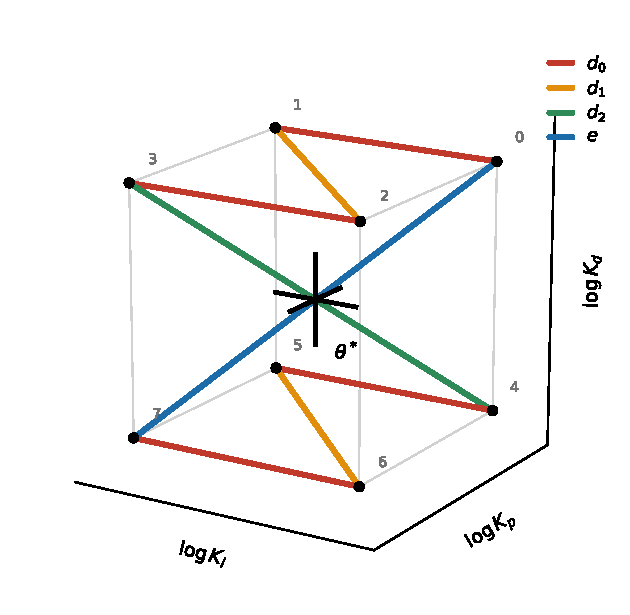
\includegraphics[width=0.9\linewidth]{fig_limit_cycle}
\caption{The limit cycle in log-gain space. One period visits the eight
corners of a cube of side $h = \log\gamma$ centered on the triple point
$\theta^*$ (black cross), in binary counting order (vertex labels); the
moves $d_0, d_1, d_2, e$ act as bit toggles and carries. The two space
diagonals ($e$, $d_2$) pass through the centre.
% NOTE: schematic drawn from the ruler ordering implied by the measured
% duty cycle; verify against a recorded terminal orbit (TODO-REGEN) and
% ideally replace/accompany with the measured orbit on P1.
}
\label{fig:cycle}
\end{figure}

\begin{table}[t]
\small
\centering
\caption{Measured share of the four moves over the last $80$ iterations,
against the prediction of Proposition~\ref{prop:balance}. Runs use the
reference implementation of \cite{Paper1} with its published (hard-count)
index. P3 at $\beta = 0.03$ reaches an exactly periodic orbit of period $8$
with move counts $(1,4,2,1)$, as Corollary~\ref{cor:period} requires.
% REGENERATED from the reference implementation (core/tuning.py), which
% reports the row that fires at each iteration. P4 is omitted: from every
% start tried it ends with a gain on a bound (boundary case), so it is not
% an interior-target run.
}
\label{tab:duty}
\begin{tabular}{llcccc}
\toprule
Plant & $\beta$ & $w_e$ & $w_{d_0}$ & $w_{d_1}$ & $w_{d_2}$ \\
\midrule
Predicted &      & $0.125$ & $0.500$ & $0.250$ & $0.125$ \\
\midrule
P1 & $0.10$ & $0.125$ & $0.487$ & $0.250$ & $0.138$ \\
P3 & $0.10$ & $0.125$ & $0.487$ & $0.263$ & $0.125$ \\
P1 & $0.03$ & $0.087$ & $0.512$ & $0.237$ & $0.163$ \\
P3 & $0.03$ & $0.125$ & $0.500$ & $0.250$ & $0.125$ \\
\bottomrule
\end{tabular}
\end{table}

\paragraph{Boundary Case} If $\theta^*$ lies outside the gain box, condition
\eqref{eq:triplepoint} cannot be satisfied and the cycle changes character.
The trajectory then settles where, for each band, either the index sits on its
threshold \emph{or} the gain sits on a bound. We call this a complementarity
point. The P2 run of the companion paper is an example. It ends with $K_d$ on
the floor of $0.01$ and indices $N = (0.11,\, 1.04,\, 1.14)$ at gains
$(0.392,\, 0.025,\, 0.01)$. What that paper describes as the rule removing
derivative action on a delay-dominant plant is exactly this boundary case.

% =====================================================================
\section{Why the Move Table Has This Form}
\label{sec:why}

The results so far describe the cycle produced by one particular table of
moves. It is natural to ask whether that table could have been chosen
differently. It could not. Once the priority order is fixed, the table of
Section~\ref{sec:rule} is the only one possible.

\begin{proposition}[The Move Table is Forced]
\label{prop:unique}
Fix the priority order of the rule. Among move tables in which
(i) every entry lies in $\{-1, 0, +1\}$, so that each gain is multiplied by
$\gamma^{\pm 1}$ or left alone; (ii) $e = (1, \dots, 1)$; and (iii) each
cut $d_k$ decreases its own gain, $d_k[k] = -1$; the staircase table
\eqref{eq:moves} is the \emph{unique} one whose balance weights
\eqref{eq:weights} coincide with the branch frequencies of the priority
logic.
\end{proposition}

\begin{proof}
Counting sign patterns, the priority logic selects $e$ on $1$ of the $2^n$
patterns and $d_k$ on $2^{\,n-k-1}$ of them, so matching requires
$e + \sum_k 2^{\,n-k-1} d_k = 0$. Coordinate $j$ of this reads
$\sum_k 2^{\,n-k-1} d_k[j] = -1$: a signed-binary representation of $-1$ with
digits in $\{-1,0,1\}$. Exactly $n$ such representations exist, indexed by the
position $m$ of the single $-1$ digit, namely $d_m[j] = -1$, $d_k[j] = +1$
for $k > m$ and $0$ for $k < m$. Hypothesis (iii) forces $m = j$, giving
$d_k[j] = +1$ for $j < k$, $-1$ for $j = k$, and $0$ for $j > k$. This is
exactly the table \eqref{eq:moves}.
\end{proof}

Hypotheses (i) and (iii) are both needed: without (iii) there are $n^n$
matching tables, and relaxing (i) to entries in $\{-2, \dots, 2\}$ gives six for
$n = 3$. The triangular shape is therefore not a design choice but the only
shape that fits the selection logic together with the balance condition. The
weights are powers of two because the selection tree is binary.

Two consequences follow. First, the matching gives a useful pairing:
$\lVert d_k \rVert = \sqrt{k+1}$, while $d_k$ occurs with frequency
$2^{-(k+1)}$, so the most frequent move is always the smallest one. Second,
the matching also says something about measurement noise. If noise removes all information from the three signs, the moves occur
at the branch frequencies, and those frequencies are the balance weights. The
expected displacement is then zero, so the iteration stays at $\theta^*$
instead of drifting away. This is a property of the move table and is proved
here by counting. A full stochastic treatment, including the case of
correlated noise where this argument no longer holds, is left to future work.

\begin{figure}[t]
\centering
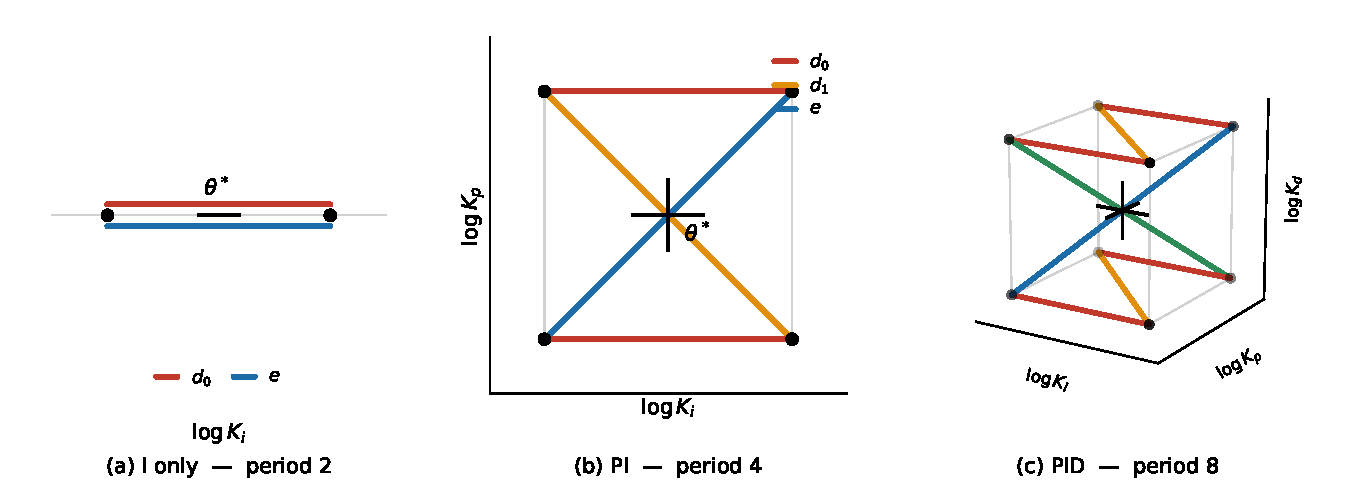
\includegraphics[width=\linewidth]{fig_limit_cycle_hierarchy}
\caption{The limit-cycle hierarchy of Remark~\ref{rem:hierarchy}: minimal
orbits for I-only ($n{=}1$, period 2), PI ($n{=}2$, period 4), and PID
($n{=}3$, period 8) tuning are binary counters on the corners of the
$n$-cube of side $h$, centered on the corresponding threshold point
$\theta^*$.}
\label{fig:hierarchy}
\end{figure}

\begin{remark}[Reduced-Order Hierarchy]
\label{rem:hierarchy}
The argument is not specific to three gains. For an $n$-gain triangular rule
with the analogous staircase moves ($e$ all $+1$; $d_k$ equal to $+1$ on the
first $k$ coordinates, $-1$ on coordinate $k$, zero after), the unique
balance has weights $w_{d_k} = 2^{-(k+1)}$ and $w_e = 2^{-n}$, the minimal
period is $2^n$, and the minimal orbit is a binary counter on the corners of
the $n$-cube: a two-point segment for pure integral tuning ($n{=}1$,
weights $\tfrac12, \tfrac12$), a square for PI ($n{=}2$, weights
$\tfrac14, \tfrac12, \tfrac14$), the cube of Fig.~\ref{fig:cycle} for PID
(Fig.~\ref{fig:hierarchy}).
% NOTE: for n=1,2 this presumes the rule keeps the same staircase move
% pattern; the companion paper defines the rule for PID only, so verify
% the reduced-order move sets against the implementation before relying
% on this remark quantitatively.
\end{remark}

% =====================================================================
\section{Cycle Size and the Choice of Step}
\label{sec:size}

The fixed-step iteration cannot converge to a point, and by
Section~\ref{sec:cycle} it should not be expected to. The practical question is
how far from the ideal target it leaves the gains. The answer is the radius of
the orbit, and Observation~\ref{obs:ruler} makes this an exact number rather
than an order of magnitude. If the switching surfaces are treated as locally
flat, every point of the cycle lies at distance $\tfrac{\sqrt{3}}{2}\, h$ from
$\theta^*$, where $h = \log\gamma$. Halving the step therefore halves the
cycle exactly. How much a measured orbit differs from a perfect cube is a
direct measure of how curved the switching surfaces are.

The cube is aligned with the gain axes, so the bound holds separately in each
coordinate. This turns the geometry into a design rule for $\beta$.

\begin{corollary}[Design Rule]
\label{cor:design}
On the terminal cycle each log-gain coordinate deviates from its value at
$\theta^*$ by exactly $h/2$, so every gain stays within the multiplicative
factor
\begin{equation}
\rho = \gamma^{1/2} = (1-\beta)^{-1/2}
\label{eq:designfwd}
\end{equation}
of its ideal value, at every iteration. To keep all three gains within a
factor $\rho$ of the target set by the plant it is therefore enough to choose
\begin{equation}
\boxed{\;\beta \;\le\; 1 - \rho^{-2}\;}
\label{eq:designrule}
\end{equation}
The bound contains no plant parameter, because the side of the cube is fixed
by the moves alone.
\end{corollary}

For an accuracy of $5\,\%$ per gain, $\rho = 1.05$ gives $\beta \le 0.093$. In
the other direction, the default $\beta = 0.1$ of the companion paper
guarantees $5.4\,\%$ per gain. That default was chosen there from experience;
here we can say what it guarantees.

Three conditions come with \eqref{eq:designrule}. It is exact when the
switching surfaces are locally flat, and curvature adds a term of order $h^2$.
It assumes that $\theta^*$ lies inside the gain box; if it does not, the
boundary case of Section~\ref{sec:cycle} applies. Under measurement noise it
holds down to the noise floor, below which the spread around $\theta^*$ is set
by the noise and not by $\beta$.

It is also worth saying which error is bounded. Equation
\eqref{eq:designrule} bounds the error in the \emph{gains}, and this bound is
the same for every plant. The corresponding error in the turn index is
$|N_k - \Nbar_k| \approx \|J_k\| \, \tfrac{\sqrt{3}}{2} h$, where $J$ is the
local Jacobian of Section~\ref{sec:structure}, and this does depend on the
plant. The indices are the measuring instrument; the gains are the result.

We measure this from far starting points, with the gains detuned by a factor
of $16$. Table~\ref{tab:schedules} gives the final log-gain distances to
$\theta^*$. With a constant $\beta$ the run reaches the cycle quickly, and the
final error of $0.074$ is the radius of that cycle. This is a few percent in
each gain, which for
% TODO-REGEN: state beta of this run and compare 0.074 against
% (sqrt(3)/2)*log(gamma) explicitly once the schedule script exists;
% also tabulate the Corollary 3 factor rho for the beta values used.
plant-floor use is indistinguishable from the target. This is the theoretical
support for the companion paper's constant-step recommendation: the fixed-step
rule is guaranteed to leave the gains within one cycle radius of a
plant-determined point, and that radius is set by $\beta$ alone.

% =====================================================================
\section{Faster Schedules}
\label{sec:accel}

A fixed step leaves a cycle of radius $\tfrac{\sqrt3}{2}h$. To do better the
step must shrink, and the obvious way is to let it shrink with the iteration
number. Table~\ref{tab:schedules} reports what this gives.

The table also lists schedules in which the step shrinks as a power of the
iteration number. These serve the analysis and are not tuning recommendations.
The schedules $n^{-1/2}$ and $n^{-3/4}$ converge to $\theta^*$ and so confirm
the center. The classical schedule $n^{-1}$ stops early, at error $0.197$. The
reason is worth stating, because it is a limit on total travel and not an
effect of noise.

\begin{lemma}[Logarithmic Travel]
\label{lem:travel}
Let $\beta_n = c/n$. The total distance covered in $n$ steps is then
$\sum_{m \le n} \log\gamma_m = -\sum_{m \le n}\log(1 - c/m) = O(\log n)$.
A target at distance $D$ therefore cannot be reached in fewer than about
$n \approx e^{D/c}$ iterations, even if every step points the right way.
\end{lemma}

With $D \approx \log 16$ per gain the required $n$ is enormous. This is the
same borderline case as in stochastic approximation, but it appears here for a
different reason. The iteration is deterministic, and $n^{-1}$ fails not
because of noise but because the total path length is too short.

\begin{table}[t]
\small
\centering
\caption{Final log-gain distance to the cycle center $\theta^*$, far start
($16\times$ detuned), regularized index.
% TODO-REGEN: from code/asymptotics/schedule_comparison.py; rows may
% be per-plant or averaged, confirm which and add to reproduce script.
}
\label{tab:schedules}
\begin{tabular}{lll}
\toprule
Schedule & Final error & Behavior \\
\midrule
$\beta$ const.           & $0.074$ & limit cycle, radius $O(h)$ \\
$\beta_n \propto n^{-1/2}$ & $0.010$ & converges (analysis) \\
$\beta_n \propto n^{-3/4}$ & $0.001$ & converges (analysis) \\
$\beta_n \propto n^{-1}$   & $0.197$ & freezes (Lemma~\ref{lem:travel}) \\
reversal-halving         & $10^{-4}$ & $36$--$98$ iters (Sec.~\ref{sec:accel}) \\
\bottomrule
\end{tabular}
\end{table}

A schedule chosen in advance is therefore either too slow or too weak. What is
needed is a step that shrinks only when shrinking it helps.


The picture of a cycle of radius $O(h)$ around a fixed center suggests such a
step directly. While the state is still traveling toward $\theta^*$ the step
should stay large. Once the state is going round the cycle, a large step no longer brings
the state closer, so it can be cut, and the cycle is halved with it. The two
situations can be told apart from the sequence of moves alone: when the state
is going round the cycle, and only then, the comparison of every band keeps
changing sign.

This gives the \emph{reversal-triggered halving} schedule. Keep $\beta$
constant until every band has reversed its direction at least once, then halve
$\beta$ and repeat. Each halving moves the state from one cube to a cube of
half the side with the same center, so the error falls geometrically and each
stage costs only a bounded number of iterations. The counter structure of
Observation~\ref{obs:ruler} also gives a natural moment to halve, since the
carry move $e$ marks the end of a full period. In the runs of
Table~\ref{tab:schedules} this schedule reaches an error of $10^{-4}$ in $36$
to $98$ iterations on the plants with an interior target. That is three orders
of magnitude better than the constant step, for a similar number of
experiments. Readers who know the learning literature will recognize the
mechanism. It is a global version of the sign-based Rprop update with
step adaptation on reversal \cite{Riedmiller1993}, and it appears naturally
here because the triangular rule also uses only signs.

We state clearly what the theory covers and what it does not. Every stage
circles a cycle with the same center $\theta^*$, and this follows from
Corollary~\ref{cor:triple}, which does not depend on the step size. That each
stage ends, that is, that every band eventually reverses, and that the radius
halves with $h$, are at present measurements that agree with
Observation~\ref{obs:ruler}. Closing this gap is the same task as proving the
cycle itself, which we discuss next.

% =====================================================================
\section{Local Structure and the Route to a Proof}
\label{sec:structure}

Two facts about the neighborhood of $\theta^*$ shape the proof. First, the
Jacobians $\partial N_j / \partial \theta_i$ of the regularized index at
$\theta^*$, computed by central differences, are nonsingular on all plants with
an interior target. Their determinants are $1.2$, $5.9$ and $4.3$ on P1, P3 and
P4. The center of the cycle is therefore locally unique.
% TODO-REGEN: add units/normalization to reproduce script.

Second, and this is what rules out the simple proof, the Jacobians are
neither diagonal nor diagonally dominant. On P1 the proportional gain changes
the band-2 index more strongly than the derivative gain does. On P4 the entry
of band~1 with respect to its own gain is negative. The intuitive picture
behind the rule, in which each move mainly repairs its own band, is therefore
wrong at the center, and an argument based on each move alone fails on two of
the three plants. Yet on all three plants the cycle forms, has the right
center, and shrinks under the faster schedule.

The explanation is that the cycle is a property of the \emph{averaged}
motion. Near $\theta^*$ the iteration switches rapidly between the four
regions, and its mean motion is the convex combination of the four velocities
weighted by the time spent in each region. This is the Filippov regularization
of the switched system \cite{Filippov1988}. The measured shares in
Table~\ref{tab:duty} are direct evidence, since the observed times are exactly
the balance weights \eqref{eq:weights}. A proof of the limit cycle should
therefore (i) show that $\theta^*$ is a stable equilibrium of the Filippov
vector field, and (ii) obtain existence, stability and the $O(h)$ radius of the
discrete cycle from a standard averaging argument. We leave this as the open
problem of the paper.

This has a practical consequence. Any scheme that treats the bands separately,
such as one step size or one momentum term per band, assumes the diagonal
structure that is missing here and should be expected to work badly. Momentum
applied to the whole move vector is the variant worth trying.

% =====================================================================
\section{Conclusions}

SPIN tuning with a fixed step ends in a limit cycle, and that cycle is now
fully described. It circles the triple point, the gain vector fixed by the
plant at which all three turn indices sit on their thresholds. Its move
frequencies $(\tfrac18, \tfrac12, \tfrac14, \tfrac18)$ follow from a single
balance condition, and the same condition over the integers gives the shortest
possible period of $8$. The cycle is realized as a binary counter on the
corners of a cube of side $\log\gamma$ centered on the triple point. If the
triple point lies outside the gain box, the cycle instead settles at a
complementarity point, as in the P2 run of the companion paper. Two tools made
the analysis possible: the balance condition, which locates the center, and the
$\varepsilon$-regularized winding index, which makes that center well defined.

The results support practice directly. Because the cube is aligned with the
gain axes, a fixed step keeps every gain within the factor $(1-\beta)^{-1/2}$
of the target set by the plant, so an accuracy $\rho$ per gain is obtained by
choosing $\beta \le 1-\rho^{-2}$. This rule contains no plant parameter, and
under it the default $\beta = 0.1$ of the companion paper guarantees
$5.4\,\%$ per gain. The reversal-triggered halving schedule shrinks the cube
geometrically and reaches $10^{-4}$ accuracy in fewer than a hundred
iterations. One theoretical step remains open: the existence and stability of
the cycle through the averaged Filippov dynamics, together with the momentum
variant that this suggests.

% =====================================================================
\small
\begin{thebibliography}{10}
\itemsep0pt

\bibitem{Paper1}
D. Pachner, P. Otta, J. Dost\'al, V. Havlena, Model-free PID tuning by
step-response inspection, submitted to J. Process Control, 2026.

\bibitem{ZN1942}
J.~G. Ziegler, N.~B. Nichols, Optimum settings for automatic controllers,
Trans. ASME 64 (1942) 759--768.

\bibitem{AstromHagglund2004}
K.~J. {\AA}str{\"o}m, T. H{\"a}gglund, Revisiting the Ziegler--Nichols
step response method for PID control, J. Process Control 14 (2004) 635--650.

\bibitem{Hjalmarsson1998}
H. Hjalmarsson, M. Gevers, S. Gunnarsson, O. Lequin, Iterative feedback
tuning: theory and applications, IEEE Control Syst. Mag. 18 (4) (1998)
26--41.

\bibitem{Killingsworth2006}
N.~J. Killingsworth, M. Krsti{\'c}, PID tuning using extremum seeking,
IEEE Control Syst. Mag. 26 (1) (2006) 70--79.

\bibitem{Riedmiller1993}
M. Riedmiller, H. Braun, A direct adaptive method for faster backpropagation
learning: the RPROP algorithm, in: Proc. IEEE Int. Conf. Neural Networks,
1993, pp. 586--591.

\bibitem{Filippov1988}
A.~F. Filippov, Differential Equations with Discontinuous Righthand Sides,
Kluwer, 1988.

\end{thebibliography}

\end{document}
